% --------------------------------------
% Document Class
% --------------------------------------
\documentclass[a4paper,11pt]{article}
% --------------------------------------



% --------------------------------------
% Use Package
% --------------------------------------


\usepackage[francais]{babel}
%\usepackage{ucs}
\usepackage[utf8]{inputenc}
\usepackage[T1]{fontenc}

\usepackage{makeidx}
\usepackage{color}
\usepackage{graphicx}
\usepackage{float}
\usepackage[hidelinks]{hyperref} 
\usepackage{geometry}
%\usepackage{lastpage}
%\usepackage{marginnote}
\usepackage{fancyhdr}
%\usepackage{titlesec}
%\usepackage{framed}
\usepackage{amsmath}
\usepackage{empheq}
\usepackage{array}
\usepackage{multicol}
\usepackage{csquotes}
%\usepackage{adjustbox}

% insert code
\usepackage{listings}

% define our color
\usepackage{xcolor}

% code color
\definecolor{ligthyellow}{RGB}{250,247,220}
\definecolor{darkblue}{RGB}{5,10,85}
\definecolor{ligthblue}{RGB}{1,147,128}
\definecolor{darkgreen}{RGB}{8,120,51}
\definecolor{darkred}{RGB}{160,0,0}

% other color
\definecolor{ivi}{RGB}{141,107,185}


\lstset{
    language=Scilab,
    captionpos=b,
    extendedchars=true,
    frame=lines,
    numbers=left,
    numberstyle=\tiny,
    numbersep=5pt,
    keepspaces=true,
    breaklines=true,
    showspaces=false,
    showstringspaces=false,
    breakatwhitespace=false,
    stepnumber=1,
    showtabs=false,
    tabsize=3,
    basicstyle=\small\ttfamily,
    backgroundcolor=\color{ligthyellow},
    keywordstyle=\color{ligthblue},
    morekeywords={include, printf, uchar},
    identifierstyle=\color{darkblue},
    commentstyle=\color{darkgreen},
    stringstyle=\color{darkred},
}


% --------------------------------------



% --------------------------------------
% Page setting
% --------------------------------------
%\pagestyle{empty}
\setlength{\headheight}{15pt}

\setcounter{secnumdepth}{3}
\setcounter{tocdepth}{2}

\makeatletter
\@addtoreset{chapter}{part}
\makeatother 

\hypersetup{         % parametrage des hyperliens
  colorlinks=true,      % colorise les liens
  breaklinks=true,      % permet les retours à la ligne pour les liens trop longs
  urlcolor= blue,       % couleur des hyperliens
  linkcolor= black,     % couleur des liens internes aux documents (index, figures, tableaux, equations,...)
  citecolor= green      % couleur des liens vers les references bibliographiques
}

% --------------------------------------

% --------------------------------------
% Information
% --------------------------------------
\title{Compte-rendu TP9 TI : Détection de contours par approches du premier ordre}
\author{Elliot VANEGUE et Gaëtan DEFLANDRE}
% --------------------------------------

\definecolor{myColor}{rgb}{0.5, 0.1, 0.75}

% --------------------------------------
% Begin content
% --------------------------------------
\begin{document}

% Set language to english
  \selectlanguage{francais}

  % Start the page counting
  \pagenumbering{arabic}

  \maketitle
  
  \mbox{}
  \newpage
  \clearpage
  
  \section*{Introduction}
  Lors de ce TP, nous allons chercher à déterminer les contours d'une image grâce aux 
  gradients de ses pixels. Ces gradients porte de nombreuse information qui peuvent
  être déterminé grâce à l'algorithme de Sobel, qui calcul le vecteur des gradients.
  
  \section{Seuillage de la norme d'un gradient}
  
  \subsection{Calcul de la norme d'un gradient par convolution}
  Nous avons dans un premier temps calculé les dérivées partielle de la fonction image dans 
  les directions horizontal et vertical. Pour cela, nous appliquons les filtres de Sobel
  $\begin{pmatrix}
     -1 & 0 & 1 \\
     -2 & 0 & 2 \\
     -1 & 0 & 1 
  \end{pmatrix}$ et 
   $\begin{pmatrix}
     -1 & -2 & -1 \\
     0 & 0 & 0 \\
     1 & 2 & 1
  \end{pmatrix}$
  Afin de calculer le gradient de chaque pixel dans la direction x et y.
  Nous obtenons ainsi une image avec les contours dont la direction est horizontal et une seconde avec les contours vertical.\\
  
  \begin{figure}[H]
  \center
   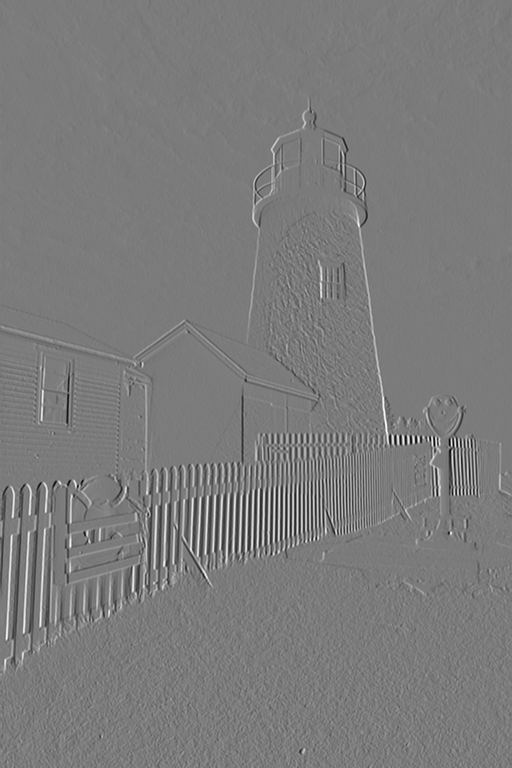
\includegraphics[width=4cm]{../lighthouse_8bits_grad_x.png}
   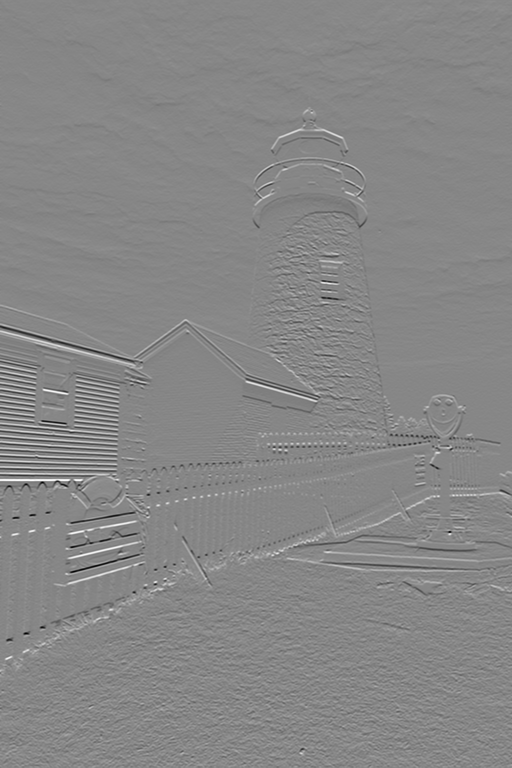
\includegraphics[width=4cm]{../lighthouse_8bits_grad_y.png}
   \caption{Images avec les contours horizontal et vertical}
  \end{figure}

  On voit sur ces deux images que les contours détecté par chaque filtre ne sont pas les mêmes
  à cause de leur direction. Grâce au valeur des pixels de ces deux images, nous calculons la norme
  des gradiants dans une nouvelle image, ce qui fera ressortir des contours de l'image.

  \begin{figure}[H]
  \center
   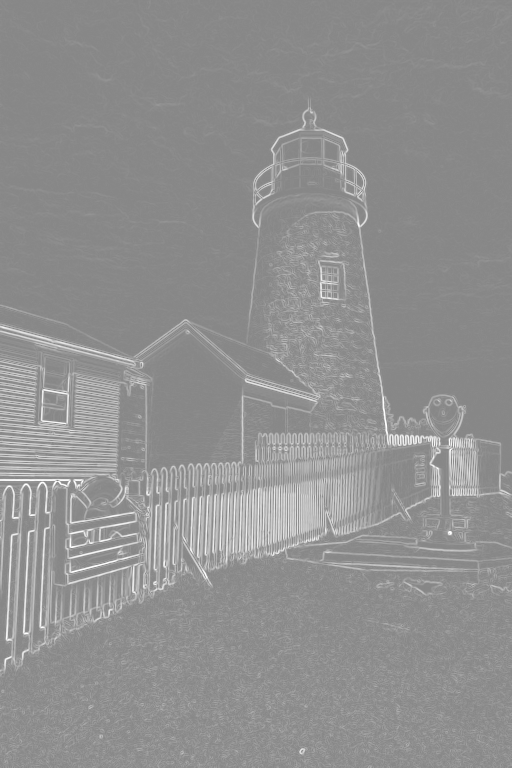
\includegraphics[width=4cm]{../norme32.png}
   \caption{Norme de l'image}
  \end{figure}
  
  On voit que la norme fait bien ressortir les contours, mais certain d'entre eux sont incomplet
  ou à l'inverse trop épais. Quand on regarde l'histogramme de l'image on voit que le minimum est 0
  et le maximum est 904 pour l'image 32 bits. Pour calculer la norme de l'image nous utilisons 
  la formule : $\sqrt{pX^2 + pY^2}$, ce qui explique la valeur assez importante du maximum. De plus,
  l'image ne comporte pas de pixel noir, car cette image comporte des valeurs négatives qui ont 
  été supprimé avec le carré des de la valeur des pixels.\\
  
  Pour obtenir le même résultat que la fonction qui calcul la norme dans ImageJ, il faut passer 
  l'image 32 bits en image 8 bits.\\
  
  \begin{figure}[H]
  \center
   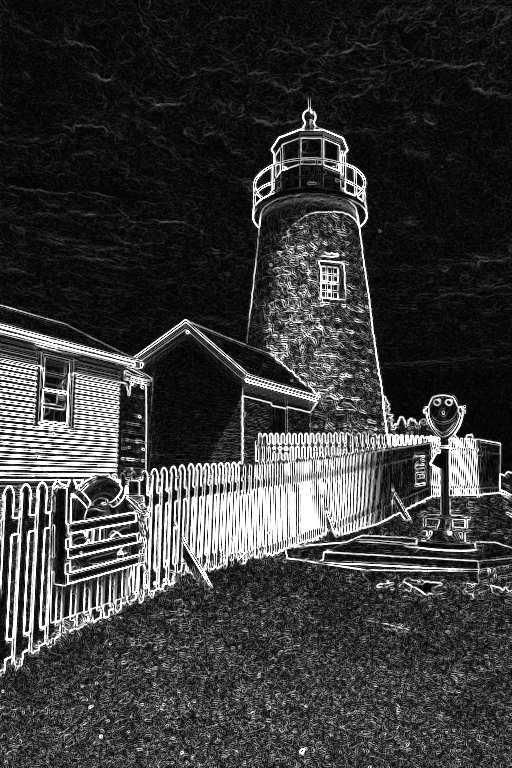
\includegraphics[width=4cm]{../norme8.png}
   \caption{Norme de l'image transformé en image 8 bits}
  \end{figure}
  
  Le résultat que nous obtenons est identique au résultat de la fonction d'ImageJ, car nous obtenons
  une image noire lorsque nous faisons la soustraction de notre résultat et celui d'ImgaJ.
  
  \subsection{Seuillage de la norme du gradient précédemment calculée}
  Grâce à l'outil ImgaeJ, nous seuillons l'image que nous avons calculer précédemment afin de la binariser.
  Nous utilisons dans un premier temps le seuillage automatique. On voit que le seuillage n'est pas excellent,
  car l'herbe est encore fort présente dans l'image et il reste quelque pixel blanc dans l'image.\\
  
  \begin{figure}[H]
  \center
   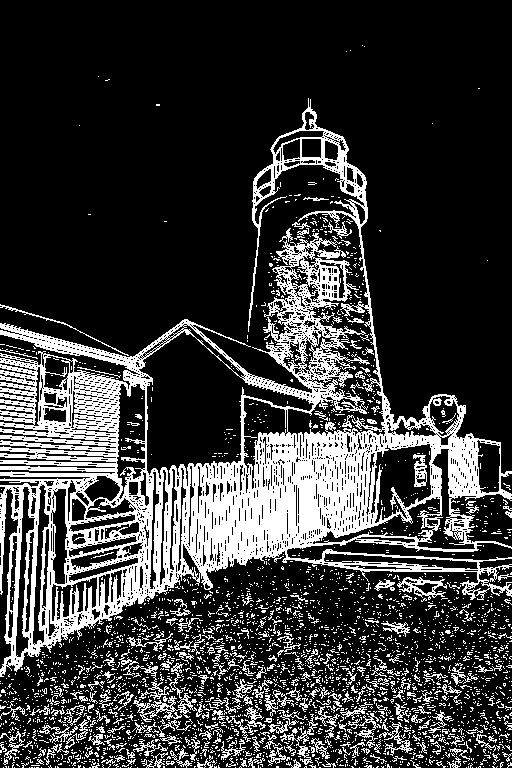
\includegraphics[width=4cm]{../binAuto.png}
   \caption{Binarisation automatique de l'image}
  \end{figure}
  
  Si nous diminuons ce seuil, le nombre de pixel blanc dans la pelouse et dans le ciel augmente. Et si
  nous augmentons le seuil, nous diminuons les pixels blanc dans les zone cité précédemment, mais nous
  perdons certains contours du phare et de la maison. Finalement, nous déterminons que le seuil le plus 
  approprié doit se trouver entre 80 et 120.\\
  
  \begin{figure}[H]
  \center
   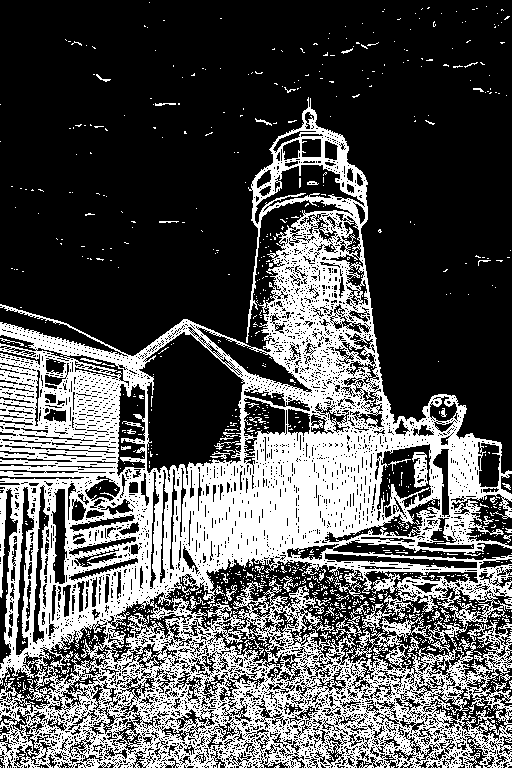
\includegraphics[width=4cm]{../bin50.png}
   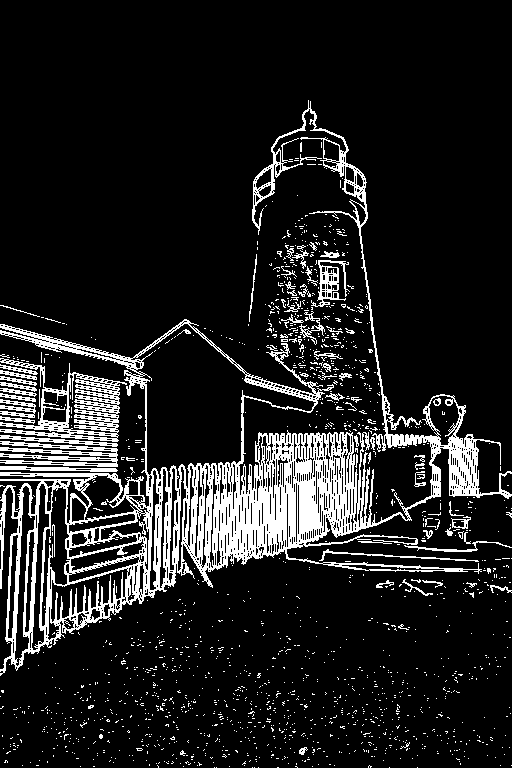
\includegraphics[width=4cm]{../bin140.png}
   \caption{Binarisation de l'image avec le seuil 50 puis 140}
  \end{figure}
  
  Afin d'affiner la détermination du seuil, nous calculons l'histogramme cumulé de l'image qui à chaque valeur
  de pixel ajoute la somme des valeurs des pixel précédent. A partir de cet histogramme, nous allons prendre
  comme seuil le pixel à partir du quel l'histogramme commence à se stabiliser. Nous allons donc prendre le pixel
  qui est à peu près à 20\% de l'histogramme, soit le pixel 100.
  
  \begin{figure}[H]
  \center
   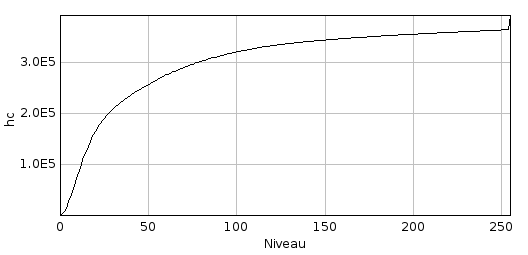
\includegraphics[width=10cm]{../histoCumul.png}
   \caption{Histogramme cumulé de l'image}
  \end{figure}
  
  \section{Détection des maxima locaux de la norme d'un gradient}
  Pour réaliser une détection des maxima locaux, nous avons besoin de calculer l'angle des gradients
  de l'image. Pour cela nous utilisons la formule suivante sur chacun des pixels : \\
  $$angle = atan2(pY, pX)/3.14*180$$
  
  Grâce à cet angle nous pouvons vérifier la valeur des deux pixels voisin qui le suive et si ces pixels
  voisin ont une valeurs plus petite que le pixel traité, alors celui-ci appartient à un contour.
  Dans ce cas on passe les voisins à 0.\\
  
  \begin{figure}[H]
  \center
   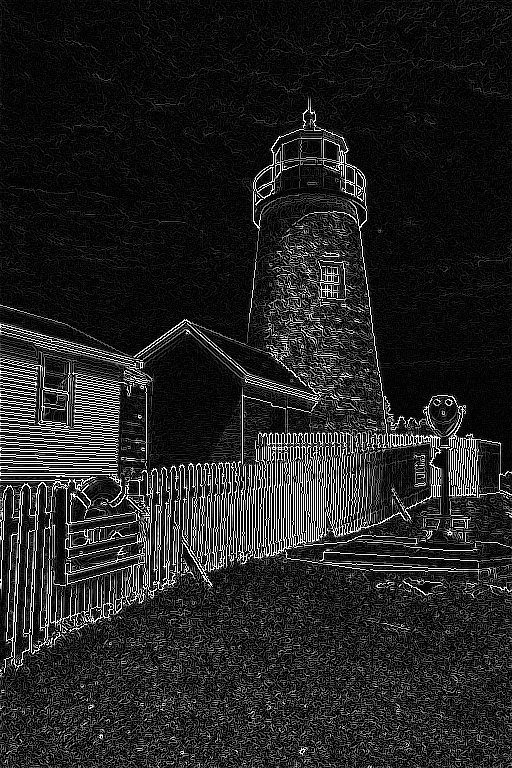
\includegraphics[width=4cm]{../maxima_locaux.png}
   \caption{Histogramme cumulé de l'image}
  \end{figure}
  
  Nous pouvons voir qu'avec cette méthode les contours sont plus fin, il ne sont composé que de un pixel
  en largeur. En revanche, cet algorithme ne supprime pas de bruit, il ne fait qu'intensifier les contours.
  
  \section{Seuillage des maxima locaux par hystérésis}
\end{document}  